\section{Sliding execution windows}

    There are two important windows that we consider in our oscilloscope, the \textit{sampling window} and the \textit{polling window}.

    \subsection{Sampling window}
    Suppose we are at time $t$, the observed (and calculated, if applicable) $\Delta$Qs at time $t$ we will display are the $\Delta$Qs obtained from the outcome instances who ended within a sampling window in the \textbf{window of time $(t-1)_{l}$ - $(t-1)_u$}, with $t-1$ equal to $t - x$, and $x$ the sampling rate. The sampling rate is how often $\Delta$Qs are calculated. \\
    This is to account for various overheads that need to be taken into consideration. They could be network overhead, the adapter overhead, C++ latency \dots Imagine multiple outcome instances that are ended at a time slightly lower but close to t, and due to the overheads the messages arrive at a time slightly higher but close to t, the outcome instance would not be taken into consideration for the calculation of a $\Delta$Q.
    
    \begin{figure}[H]
        \begin{center}
            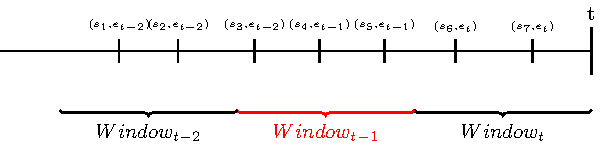
\includegraphics{tikz/window.pdf}
        \end{center}
    \end{figure}
    
    The sampling window then advances every $x$ seconds, setting the new window: 
    \begin{center}
        From: $(t-1)_l$, $(t-1)_u$ $\xrightarrow{t + 1}$ $t_l, t_u$. \\
        Where: $t_l = (t-1)_u$ and $t_u = (t-1)_u + x$ 
    \end{center}
    
    The $\Delta$Qs which are observed and calculated in a sampling window are not precise, this is why we need to introduce the polling window.

    \subsection{Polling window (Observing multiple $\Delta$Qs over a time interval)}
        The polling window is the window of $\Delta$Qs which are stored to keep a snapshot of the system over time and over which confidence bounds are calculated. The polling window serves to improve the precision of the $\Delta$Q measurement.
        
        Suppose we are at time $t = 0$, the polling window will have 0 $\Delta$Qs. As the sampling window advances, more $\Delta$Qs are sampled, which in turn are added to the snapshot and to the confidence bounds.

        The limit of $\Delta$Qs for a polling window (subsequently snapshots and confidence bounds) is 30 $\Delta$Qs. At $t= 31$, the older $\Delta$Qs will be removed from the polling window and in turn from the snapshots and confidence bounds. Newer sampled $\Delta$Qs will be added, keeping the limit of $\Delta$Qs in a polling window to 30.

